\begin{figure*}[htbp]
  \centering
  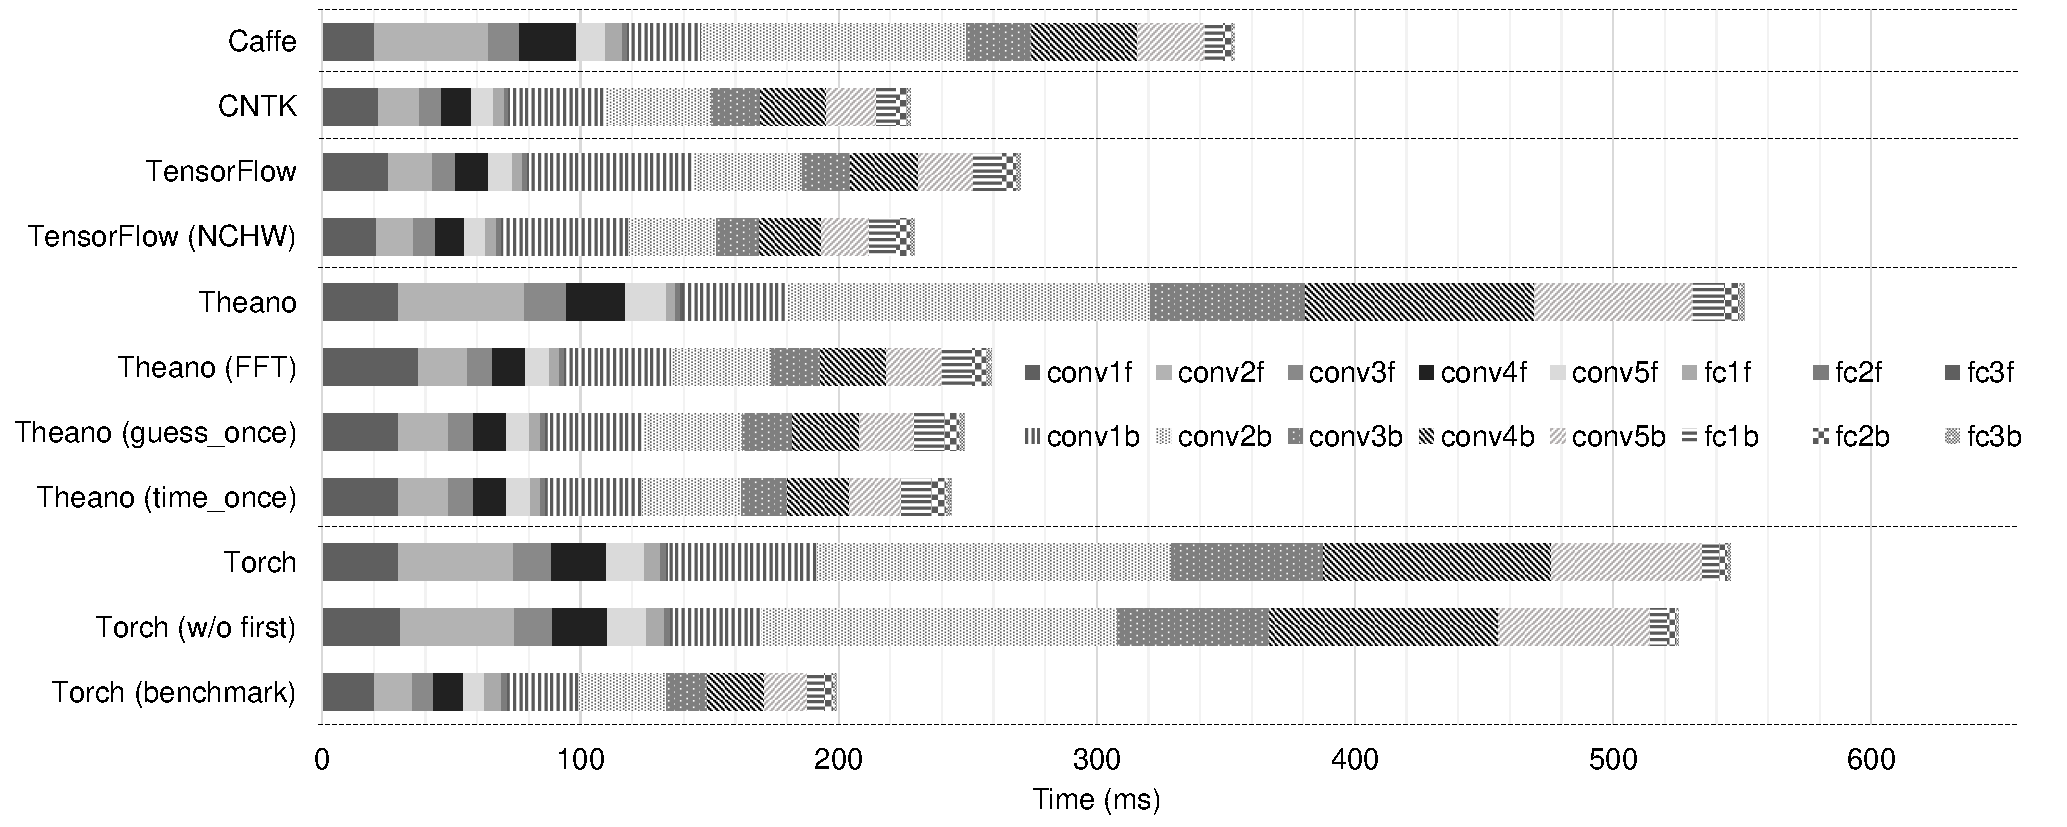
\includegraphics[width=\linewidth]{./figures/time_frameworks}
  \caption{%
The execution time of training AlexNet with a batch of input images for different deep learning frameworks. 
\label{fig_time_frameworks}
  }
\end{figure*}

%A = Caffe, B = TensorFlow, C = TensorFlow (NCHW tensor), D = Theano, E = Theano (FFT), F = Theano (guess\_once), G = Theano (time\_once), H = Torch, I = Torch (no backward propagation in the first layer), J = Torch (FFT), K = Torch (benchmarking) 

\section{Charactrization on a Single GPU}
\label{sec:singlGPU}
In this section, we characterize the five deep learning frameworks on a single GPU. The measurement of the layer-wise execution time of the AlexNet model for each framework is shown in Figure~\ref{fig_time_frameworks}. The batch size of 256 was used in the experiment. The string in parentheses after the framework name stands for the framework configuration when the AlexNet model is built. No parentheses means the default options. A bar shows the breakdown of the total execution time into that of each layer. A layer name suffixed with \textsf{f} stands for the forward computation stage, and \textsf{b} for the backward computation stage.

\subsection{Options for Convolution Algorithms}
{\bf Caffe}. Caffe does not have any explicit option to choose convolution algorithms. Instead, it exploits cuDNN's heuristics that try to determine the best suited algorithm under the given specification of the model. Surprisingly, Caffe does not have an appropriate memory management technique yet. As a result, algorithms that require a smaller memory space, such as GEMM and Winograd, can be inappropriately selected resulting in low performance even if Caffe exploits cuDNN's heuristics. 

{\bf TensorFlow}. TensorFlow also does not provide any option to choose convolution algorithms. Unlike Caffe, however, it executes all available algorithms in the first run by itself. Then, the fastest algorithm for each layer is executed in subsequent runs. The FFT algorithm is chosen for all the convolution layers except \textsf{conv1}, where FFT cannot be used because of the stride size (4). Since the set of algorithms that can be chosen is fixed and hardwired, recently added options of cuDNN R5.1 are not included in the set.

{\bf Theano}. On the other hand, Theano provides full accesses to the choices of convolution algorithms. Users can specify a specific convolution algorithm globally or in a layer-by-layer manner. There are two types of GEMM implementations in cuDNN: explicit and implicit. Theano selects the explicit GEMM by default. When a convolution algorithm is given as a global option, and the algorithm does not match the condition for a layer, the implicit GEMM is chosen as a fallback for the layer. However, the implicit GEMM is usually slower than the explicit GEMM. Thus, it is better to give layer-wise option to make Theano not to choose the implicit GEMM. \textsf{Theano (FFT)} in Figure~\ref{fig_time_frameworks} stands for the AlexNet model built by Theano with a global option for the FFT algorithm. However, \textsf{conv1} cannot use the FFT algorithm because of its stride size. Instead, the implicit GEMM is chosen for \textsf{conv1}. This is the reason why \textsf{conv1} of \textsf{Theano (FFT)} in Figure~\ref{fig_time_frameworks} is slower than those of \textsf{Theano (guess\_once)}, \textsf{Theano (time\_once)}, and even \textsf{Theano}. 

Unlike Caffe, Theano properly exploits cuDNN's heuristics when the \textsf{guess\_once} option is given. The \textsf{guess\_once} option makes Theano behave like Caffe where cuDNN's heuristics determine the best suited algorithm. The \textsf{time\_once} option in Theano exploits cuDNN's another functionality that executes all available convolution algorithms and choose the fastest one. Unlike TensorFlow, the set of algorithms in Theano is not hardwired. When the \textsf{time\_once} option is on, Theano uses GEMM in the first layer. It uses FFT or Winograd for the rest of the convolution layers. When the \textsf{guess\_once} option is on, the selection of an algorithm for each layer is slightly different from \textsf{time\_once}, but the execution time is almost the same as that of \textsf{time\_once}. This implies that cuDNN's heuristics are quite reliable.

\begin{table}[htbp]
\centering
\caption{Other GPU Kernels}
\label{table_misc_kernel}
\begin{scriptsize}
\begin{tabular}{|l|l|l|l|l|l|}
\hline\hline
           & Caffe    & CNTK    & TensorFlow & Theano  & Torch \\ \hline\hline
Bias       & cuDNN    & CNTK    & TensorFlow & Theano  & cuDNN \\ \cline{2-6} 
addition   & 2.64 ms  & 4.74 ms & 2.84 ms    & 7.88 ms & 2.63 ms  \\ \hline\hline
ReLU       & cuDNN    & CNTK    & Eigen      & Theano  & cuDNN \\ \cline{2-6}
activation & 2.56 ms  & 2.26 ms & 2.43 ms    & 4.59 ms & 2.56 ms  \\ \hline
\end{tabular}
\end{scriptsize}
\end{table}

Although Theano executes the fastest algorithm for convolution computation, it does not have the fastest convolution layer because of other computations for bias addition and ReLU activation. Table~\ref{table_misc_kernel} lists computations included in a convolution layer, but not directly participate in convolution. It also shows the sources of the implementations. Their execution time is measured in \textsf{conv1}. Theano uses GPU implementations that are dynamically compiled at run time, and they are noticeably slower than those in other frameworks.

{\bf Torch}. Like Theano, Torch provides a full control over algorithm choices. Its cuDNN backend, cudnn.torch, has the \textsf{cudnn.benchmark} option that is the same as \textsf{time\_once} in Theano. When \textsf{benchmark} option is on, Torch is the fastest among the frameworks. 

{\bf CNTK}. CNTK does not provide any options for algorithm choices. Instead, similar to Theano and Torch, CNTK uses cuDNN's functionality to choose the fastest kernel by executing all the convolution algorithms. CNTK is not the fastest though because its bias addition implementation makes it run slow.

\subsection{Effect of Data Layout}
We also find that data layout affects performance a lot. The most noticeable one is the tensor format.
Caffe, CNTK, Theano, and Torch use the $NCHW$ 4D tensor format mentioned in Section~\ref{sec:CNN}. 

Even though TensorFlow supports the $NCHW$ format, it seems to prefer the $NHWC$ format. Sample code in TensorFlow uses the $NHWC$ format, and many function in TensorFlow, such as conv2d, uses it as the default argument format. Since channel data are stored in the last dimension in the $NHWC$ format, the performance will be better off using it when there are innermost channel-wise operations. However, some convolution algorithms, such as FFT, in cuDNN support only $NCHW$ format. Moreover, by default, TensorFlow performs conversion between $NHWC$ and $NCHW$ even if it uses algorithms that support the $NHWC$ format. Thus, using the $NHWC$ tensor format introduces significant conversion overhead before and after convolution computation. In Figure~\ref{fig_time_frameworks}, just changing the tensor format from $NHWC$ to $NCHW$ leads to about 15\% performance improvement. 

\subsection{Unnecessary Backpropagation}
\textsf{conv1} in AlexNet does not have its previous layer. Thus, there is no need to perform the backpropagation of gradients computed in \textsf{conv1} . Caffe, CNTK, and Theano automatically omit the backpropagation. Torch omits it when \textsf{gradInput} of \textsf{conv1}  is set to nil.

On the contrary, TensorFlow always performs the backpropagation of \textsf{conv1}  to prevent non-reproducibility caused by race conditions (gate\_gradients parameter in tf.train.Optimizer.compute\_gradients). This makes TensorFlow slower than Torch even if Torch has almost the same algorithms as those of TensorFlow for the convolution layers. For this reason, in Figure~\ref{fig_time_frameworks}, we see that the execution time of \textsf{conv1b} in \textsf{TensorFlow (NCHW)} is significantly different from that in \textsf{Torch (benchmark)}. However, the backpropagation can be disabled at the expense of reproducibility and the accuracy of gradient computation, although we left it enabled in our experiment for Figure~\ref{fig_time_frameworks}.


Overall, we observe that slight changes in framework options result in large performance differences. Options for convolution algorithm choices, data layout, and disabling useless backpropagation are most influential. We can increase the speed of training a CNN model up to 2X by just changing framework options. We do not need to modify the source code of the framework at all. For example, \textsf{Theano (FFT)}, \textsf{Theano (guess\_once)}, and \textsf{Theano (time\_once)} are 2X faster than \textsf{Theano}. \textsf{Torch (benchmark)} are also 2X faster than \textsf{Torch}.

%그 외 사소한 것으로 텐서에 네트워크 입력을 feed_dict로 주면 CPU 복사가 일어나서 매우 느리므로 FixedLengthRecordReader 등으로 주는게 좋다.
%https://github.com/tensorflow/tensorflow/issues/2919

%https://github.com/BVLC/caffe/blob/rc3/src/caffe/layers/cudnn_conv_layer.cpp#L113
%https://github.com/tensorflow/tensorflow/blob/v0.10.0rc0/tensorflow/core/kernels/conv_ops.cc#L460
%https://github.com/tensorflow/tensorflow/blob/v0.10.0rc0/tensorflow/stream_executor/cuda/cuda_dnn.cc#L933
%https://github.com/Theano/Theano/blob/rel-0.8.2/theano/sandbox/cuda/dnn.py#L285
%https://github.com/Theano/Theano/blob/rel-0.8.2/theano/sandbox/cuda/dnn_fwd.c#L227
%https://github.com/soumith/cudnn.torch/blob/R5/SpatialConvolution.lua#L166

